\documentclass[a4paper]{article}
\usepackage[utf8]{inputenc}


%=-=-=-=-=-=-=-=-=-=-=-=-=-=-=-=-=-=-=-=-=-=-=-=-=-=-=-=-=-=-=-=-=-=-=-=-=-=-=-=-
% PREAMBLE
%=-=-=-=-=-=-=-=-=-=-=-=-=-=-=-=-=-=-=-=-=-=-=-=-=-=-=-=-=-=-=-=-=-=-=-=-=-=-=-=-

%%%%%%%%%%%%%%%%%%%%%%%%%%%%%%%%%%%%%%%%%%%%%%%%%%%%%%%%%%%%%%%%%%%%%
% Important styling notes
%%
% For now, to include img.jpg in img/path/to/img.jpg, just use:
% path/to/img.jpg - for details see style.tex
%=-=-=-=-=-=-=-=-=-=-=-=-=-=-=-=-=-=-=-=-=-=-=-=-=-=-=-=-=-=-=-=-=-=-=-=-=-=-=-=-
% Packages
%%
%\usepackage{fullpage} % Package to use full page
\usepackage[top=1in,bottom=1in,left=1in,right=0.7in,heightrounded]{geometry}

\usepackage{parskip}                    % Package to tweak paragraph skipping
\usepackage{amsmath}                    % standard
\usepackage{amssymb}                    % standard - Double R symbol etc.
\usepackage{hyperref}
\usepackage{amsthm}                     % standard - theorem, definition, etc.
\usepackage{multicol}                   % multiple columns for numbering
\usepackage{enumitem}                   % standard - enumerate styles
\usepackage[utf8]{inputenc}
\usepackage{scrextend}                  % indentation
\usepackage{graphicx}                   % standard - add figures
\usepackage{float}                      % standard - figure position, use [H] option
\usepackage{pifont}                     % symbols
\usepackage{gensymb}                    % degree symbol \degree
\usepackage{xcolor}                     % bg color
\hypersetup{
    colorlinks,
    linkcolor={black!50!black},
    citecolor={blue!50!black},
    urlcolor={blue!80!black}
}
\usepackage{framed}                     % bg color
\usepackage[T1]{fontenc}                % small caps
\usepackage{sectsty}                    % headings colour
\usepackage{mathtools}                  % Loads amsmath
\usepackage{amsthm,thmtools,xcolor}     % coloured theorem
\usepackage[toc,page]{appendix}         % reference to appendix
%\usepackage{titlesec}                   % change chapter, section, etc. formats
\usepackage{xifthen}                    % if, else
\usepackage{etoolbox}
% format numbering in theorem, lemma, etc. environment
\AtBeginEnvironment{theorem}{\setlist[enumerate, 1]{font=\upshape,  wide=0.5em, before=\leavevmode}}
\AtBeginEnvironment{lemma}{\setlist[enumerate, 1]{font=\upshape,  wide=0.5em, before=\leavevmode}}
\usepackage[letterspace=150]{microtype} % \textls{<letterspaced text>} % 0 <= letterspace <= 1000, 1000 = M space
\usepackage{letltxmacro}                % renew commands?
\usepackage{minted}                     % package to list code
    % otherwise minted goes off the page
    \setmintedinline{breaklines}
\usepackage{subfig}
\usepackage{eso-pic}                    % title page bg pic
\usepackage{varwidth}
\PassOptionsToPackage{svgnames}{xcolor}
\usepackage{fontawesome}                % \faQuestionCircle
\usepackage{marvosym}                   %\Pointinghand
\usepackage{mdframed}                   % easy outline frames
\usepackage[many]{tcolorbox}            % colour box for theorem styles
\usepackage{array,booktabs,calc} % table figs and text
\usepackage{comment}                    % \begin{comment}
\usepackage{fancyhdr}                   % page headings
\usepackage{mdframed}                   % boxes
\usepackage[backend=biber,sorting=none,style=ieee]{biblatex}
\usepackage{caption}
%%% caption options {
%\DeclareCaptionFont{white}{\color{white}}
\DeclareCaptionFormat{listing}{\colorbox{magenta!30!gray}{\parbox{\textwidth}{#1#2#3}}}
\captionsetup[lstlisting]{format=listing,labelfont={bf,small},textfont=small,skip=-1pt}
%%% }
\addbibresource{bibliography.bib}
\usepackage{url}
\usepackage{textcomp}
\usepackage[makeroom]{cancel}            % crossed symbols
\usepackage{algorithm}
\usepackage[noend]{algpseudocode}
\usepackage{tikz}
\usetikzlibrary{arrows.meta,positioning,quotes} % arrows and nodes in tikz
\usepackage{marginnote}
\usepackage{pgfplots}
\usepackage{pstricks-add,pst-slpe}  % for fancy tikz arrows
%\usepackage{titlesec}                   % title style
\usepackage{lmodern}                    % a font
\usepackage{titletoc} % Required for manipulating the table of contents
\usepackage{titlesec} % Allows customization of titles
\usepackage{fouriernc} % Use the New Century Schoolbook font
\usepackage{booktabs} % things in page margins
\usepackage{stmaryrd } % \varoast
\usepackage{listings} % code listings
\usepackage{longtable} % table across multiple pages
\usepackage{styles/nasm/lang}  % include custom language for NASM assembly.
\usepackage{styles/nasm/style} % include custom style for NASM assembly.



%% extra comments that I don't know where they belong:
% list of ding tags: http://willbenton.com/wb-images/pifont.pdf

%=-=-=-=-=-=-=-=-=-=-=-=-=-=-=-=-=-=-=-=-=-=-=-=-=-=-=-=-=-=-=-=-=-=-=-=-=-=-=-=-
% Colours for various things
%%


\definecolor{shadecolor}{rgb}{1.,0.933,0.96} % bg color, r,g,b <= 1
\definecolor{medium_blue}{RGB}{60,125,190}
\definecolor{dark_blue}{RGB}{25,60,85}
\definecolor{dark_red}{RGB}{77,16,16}
\definecolor{LightPink}{rgb}{0.92.,0.8,0.84} % bg color, r,g,b <= 1
\definecolor{LighterPink}{rgb}{1.,0.94,0.97} % bg color, r,g,b <= 1
\definecolor{LightestPink}{rgb}{1.,0.95,0.99} % bg color, r,g,b <= 1
\definecolor{DarkestPink}{rgb}{0.36, 0.0, 0.18}
\definecolor{DarkerPink}{rgb}{0.41, 0.0, 0.21}
\definecolor{DarkPink}{rgb}{0.55, 0.05, 0.37}
\definecolor{lightestestpink}{RGB}{255,248,252}
\definecolor{codegray}{rgb}{0.5,0.5,0.5}
\definecolor{codegrayblue}{rgb}{0.35,0.35,0.47}



%=-=-=-=-=-=-=-=-=-=-=-=-=-=-=-=-=-=-=-=-=-=-=-=-=-=-=-=-=-=-=-=-=-=-=-=-=-=-=-=-
% Define my own theorem styles
%%

% "base" styles
\declaretheoremstyle[
  headfont=\color{DarkPink}\bfseries,
  bodyfont=\itshape,
]{colored}

\declaretheoremstyle[
  headfont=\color{DarkPink}\bfseries,
  bodyfont=\normalfont,
]{colored_upright}

% theorems (corollaries, etc) themselves, inherit from my style above
% Usage:
% \begin{theorem} \end{theorem}, \begin{lemma} \end{lemma}, ...
\declaretheorem[
	numberwithin=section,
 	style=colored,
	name=\textsc{Theorem},
]{theorem}

\tcolorboxenvironment{theorem}{
  boxrule=0pt,
  boxsep=2pt,
  colback={magenta!25!white},
  colframe=DarkPink,
  enhanced jigsaw, 
  borderline west={2pt}{0pt}{DarkPink},
  sharp corners,
  before skip=5pt,
  after skip=5pt,
  breakable,
  right=0mm % for equations
}

\declaretheorem[
	numberwithin=section,
 	style=colored,
	name=\textsc{Corollary},
]{corollary}

\tcolorboxenvironment{corollary}{
  boxrule=0pt,
  boxsep=1pt,
  colback={magenta!10!white},
  colframe=DarkPink,
  enhanced jigsaw, 
  borderline west={2pt}{0pt}{DarkPink},
  sharp corners,
  before skip=5pt,
  after skip=5pt,
  breakable,
  right=0mm % for equations
}

\declaretheorem[
	numberwithin=section,
	style=colored,
	name=\textsc{Lemma},
]{lemma}

\tcolorboxenvironment{lemma}{
  boxrule=0pt,
  boxsep=1pt,
  colback={magenta!10!white},
  colframe=DarkPink,
  enhanced jigsaw, 
  borderline west={2pt}{0pt}{DarkPink},
  sharp corners,
  before skip=5pt,
  after skip=5pt,
  breakable,
  right=0mm % for equations
}

\declaretheorem[
	numberwithin=section,
	style=colored,
	name=\textsc{Definition},
]{definition}

\tcolorboxenvironment{definition}{
  boxrule=0pt,
  boxsep=1pt,
  colback={magenta!25!white},
  colframe=DarkPink,
  enhanced jigsaw, 
  borderline west={2pt}{0pt}{DarkPink},
  sharp corners,
  before skip=5pt,
  after skip=5pt,
  breakable,
  right=0mm % for equations
}

\declaretheorem[
	numberwithin=section,
  	style=colored,
  	name=\textsc{Example},
]{exmp}

\declaretheorem[
	numberwithin=section,
  	style=colored,
  	name=\textsc{Solution},
]{soln}

%%% code listings
\lstdefinestyle{code1}{
    backgroundcolor=\color{lightestestpink},   
    commentstyle=\color{codegrayblue},
    keywordstyle=\color{DarkerPink},
    numberstyle=\tiny\color{codegray},
    stringstyle=\color{black!40!cyan},
    basicstyle=\small\ttfamily,
    breakatwhitespace=false,
    breaklines=true,        
    captionpos=t,             
    keepspaces=true,        
    numbers=left,           
    numbersep=5pt,
    showspaces=false, 
    showstringspaces=false,
    showtabs=false,
    tabsize=4
}

\lstset{style=code1}

%=-=-=-=-=-=-=-=-=-=-=-=-=-=-=-=-=-=-=-=-=-=-=-=-=-=-=-=-=-=-=-=-=-=-=-=-=-=-=-=-
% Headers (size, font, colour)
%%




\makeatletter
\renewcommand{\@seccntformat}[1]{\llap{\textcolor{DarkestPink}{\csname the#1\endcsname}\hspace{1em}}}                    
\renewcommand{\section}{\@startsection{section}{1}{\z@}
{-4ex \@plus -1ex \@minus -.4ex}
{1ex \@plus.2ex }
{\normalfont\large\sffamily\bfseries\textcolor{DarkestPink}}}
\renewcommand{\subsection}{\@startsection {subsection}{2}{\z@}
{-3ex \@plus -0.1ex \@minus -.4ex}
{0.5ex \@plus.2ex }
{\normalfont\sffamily\bfseries\textcolor{DarkestPink}}}
\renewcommand{\subsubsection}{\@startsection {subsubsection}{3}{\z@}
{-2ex \@plus -0.1ex \@minus -.2ex}
{.2ex \@plus.2ex }
{\normalfont\small\sffamily\bfseries\textcolor{DarkestPink}}}                        


%=-=-=-=-=-=-=-=-=-=-=-=-=-=-=-=-=-=-=-=-=-=-=-=-=-=-=-=-=-=-=-=-=-=-=-=-=-=-=-=-
% Numberings, counters and spacings
%%
\numberwithin{equation}{section} % section number in eq/s
\setlength{\jot}{7pt} % spacing in split, gathered env/s



%% Custom examples
%% Output - Example 1,2,...
\newcounter{example}
\newenvironment{example}[1][]{\refstepcounter{example}\par\medskip
   \textbf{Example~\theexample. #1} \rmfamily}{\medskip}
%%%%%%%%%%%% End of unused %%%%%%%%%%%%



%=-=-=-=-=-=-=-=-=-=-=-=-=-=-=-=-=-=-=-=-=-=-=-=-=-=-=-=-=-=-=-=-=-=-=-=-=-=-=-=-
% Paths
%%
\graphicspath{ {./img/} } % figures' path - can look up files directly from there


%=-=-=-=-=-=-=-=-=-=-=-=-=-=-=-=-=-=-=-=-=-=-=-=-=-=-=-=-=-=-=-=-=-=-=-=-=-=-=-=-
% User defined macros (math mode)
%%


% Curly braces under text. Usage: \myunderbrace{upper}{lower}
\newcommand{\myunderbrace}[2]{\mathrlap{\underbrace{\phantom{#1}}_{#2}} #1}
\newcommand{\setR}{\mathbb{R}} % \ouble R
\newcommand{\setRn}{\mathbb{R}^n} %  double R^n
\newcommand{\setN}{\mathbb{N}} % double N
\newcommand{\setZ}{\mathbb{Z}} % double Z
\let\oldemptyset\emptyset
\let\emptyset\varnothing % nice - looking empty set symbol
\newcommand{\fancyN}{\mathcal{N}} % null space
\newcommand{\fancyR}{\mathcal{R}} % range

\newcommand{\bx}{\textbf{x}}
\newcommand{\by}{\textbf{y}}
\newcommand{\bb}{\textbf{b}}
\newcommand{\bA}{\textbf{A}}
\newcommand{\bB}{\textbf{B}}
\newcommand{\bI}{\textbf{I}}
% double bars as in norm
\newcommand{\norm}[1] {\lVert #1 \rVert} 
\newcommand{\trans}[1]{#1^{\top}}

\newcommand{\mean}[1]{\bar{#1}}
\newcommand{\var}{\sigma^2}

\newcommand{\partdevx}[1]{\frac{\partial #1}{\partial x}}
\newcommand{\partdevxx}[1]{\frac{\partial #1}{\partial x}}
\newcommand{\partdevxn}[1]{\frac{\partial^n #1}{\partial x^n}}
\newcommand{\partdevy}[1]{\frac{\partial #1}{\partial x}}
\newcommand{\partdevyy}[1]{\frac{\partial #1}{\partial y}}
\newcommand{\partdevyn}[1]{\frac{\partial^n #1}{\partial y^n}}

% text above = symbol
\newcommand{\overeq}[1]{\ensuremath{\stackrel{#1}=}} 
\newcommand{\greatersmaller}{%
  \mathrel{\ooalign{\raisebox{.6ex}{$>$}\cr\raisebox{-.6ex}{$<$}}}
} % greater and smaller symbols on top of each other, same line

%=-=-=-=-=-=-=-=-=-=-=-=-=-=-=-=-=-=-=-=-=-=-=-=-=-=-=-=-=-=-=-=-=-=-=-=-=-=-=-=-
% User defined macros (non math)

\newcommand{\qedblack}{$\hfill\blacksquare$} % black square end of line
\newcommand{\qedwhite}{\hfill \ensuremath{\Box}} % white square end of line
\newcommand{\hquad}{\hskip0.5em\relax}% half quad space
%\newcommand{\TODO}{\textcolor{red}{\bf TODO!}\;}

\newcommand{\TODO}[1][]{%
    \ifthenelse{\equal{#1}{}}{\textcolor{red}{\bf TODO!}\;}{\textcolor{red}{\textbf {TODO:} #1}\; }%
}
\newcommand{\B}[1]{\textbf{\textup{#1}}} % bold and upright
\renewcommand{\labelitemi}{\scriptsize$\textcolor{DarkPink}{\blacksquare}$} % itemize - squares instead of bullets
\newcommand{\emphasis}[1]{\textls{#1}}

\LetLtxMacro{\originaleqref}{\eqref}
\renewcommand{\eqref}{Eq.~\originaleqref}
\renewcommand*{\eqref}[1]{Eq.~\originaleqref{#1}}





% background images
%%%%%%%
\newcommand\BackgroundPic{%
\put(0,0){%
\parbox[b][\paperheight]{\paperwidth}{%
\vfill
%\centering

\includegraphics[width=0.125\paperwidth,height=\paperheight,%
]{img/background_02.png}% use ,keepaspectratio
\vfill
}}}
%%%%%%%
% end of background image
%%%%%%%%%%%%%% my own frame
\newmdenv[topline=false,bottomline=false]{leftrightbox}
%%%%%%%%%%%%% end
%%%%%%%%%%%%% my own comment
\newcommand{\mycomment}[1]{\begin{leftrightbox}\Pointinghand~\textbf{Comment:}~#1 \end{leftrightbox}}
%%%%%%%%%%%%% end
% my custom note https://tex.stackexchange.com/questions/301993/create-custom-note-environment-with-tcolorbox
\newmdenv[
    topline=false,
    bottomline=false,
    rightline=false,
    innerrightmargin=0pt
]{siderule}
\newenvironment{mynote}%
    {\begin{siderule}\textbf{\Pointinghand~Note:}}
    {\end{siderule}}
%%%%%%%%%%%%% my own box
\newcommand{\boxone}[1]{\begin{tcolorbox}[colback = LighterPink,colframe=LightPink]
#1
\end{tcolorbox}}
%%%%%%%%%%%%% end

\let\oldemptyset\emptyset
\let\emptyset\varnothing
%algorithmic
\algdef{SE}[DOWHILE]{Do}{doWhile}{\algorithmicdo}[1]{\algorithmicwhile\ #1}%






\begin{document}
%=-=-=-=-=-=-=-=-=-=-=-=-=-=-=-=-=-=-=-=-=-=-=-=-=-=-=-=-=-=-=-=-=-=-=-=-=-=-=-=-
% GLOBAL STYLES (DOCUMENT SCOPE)
%=-=-=-=-=-=-=-=-=-=-=-=-=-=-=-=-=-=-=-=-=-=-=-=-=-=-=-=-=-=-=-=-=-=-=-=-=-=-=-=-
% caption: Figure 1 -> <bold> Fig. 1 </bold>
\captionsetup[figure]{labelfont={bf},labelformat={default},labelsep=period,name={Fig.}}


%=-=-=-=-=-=-=-=-=-=-=-=-=-=-=-=-=-=-=-=-=-=-=-=-=-=-=-=-=-=-=-=-=-=-=-=-=-=-=-=-
% TITLE PAGE
%=-=-=-=-=-=-=-=-=-=-=-=-=-=-=-=-=-=-=-=-=-=-=-=-=-=-=-=-=-=-=-=-=-=-=-=-=-=-=-=-
%%%%%%%%%%%%%%%%%%%%%%%%%%%%%%%%%%%%%%%%%
% Formal Book Title Page
% LaTeX Template
% Version 2.0 (23/7/17)
%
% This template was downloaded from:
% http://www.LaTeXTemplates.com
%
% Original author:
% Peter Wilson (herries.press@earthlink.net) with modifications by:
% Vel (vel@latextemplates.com)
%
% License:
% CC BY-NC-SA 3.0 (http://creativecommons.org/licenses/by-nc-sa/3.0/)
% 
% This template can be used in one of two ways:
%
% 1) Content can be added at the end of this file just before the \end{document}
% to use this title page as the starting point for your document.
%
% 2) Alternatively, if you already have a document which you wish to add this
% title page to, copy everything between the \begin{document} and
% \end{document} and paste it where you would like the title page in your
% document. You will then need to insert the packages and document 
% configurations into your document carefully making sure you are not loading
% the same package twice and that there are no clashes.
%
%%%%%%%%%%%%%%%%%%%%%%%%%%%%%%%%%%%%%%%%%

%----------------------------------------------------------------------------------------
%	PACKAGES AND OTHER DOCUMENT CONFIGURATIONS
%----------------------------------------------------------------------------------------



%----------------------------------------------------------------------------------------
%	TITLE PAGE
%----------------------------------------------------------------------------------------



\begin{titlepage} % Suppresses headers and footers on the title page

	\centering % Centre everything on the title page
	
	\scshape % Use small caps for all text on the title page
	
	\vspace*{\baselineskip} % White space at the top of the page
	
	%------------------------------------------------
	%	Title
	%------------------------------------------------
	
	\rule{\textwidth}{1.6pt}\vspace*{-\baselineskip}\vspace*{2pt} % Thick horizontal rule
	\rule{\textwidth}{0.4pt} % Thin horizontal rule
	
	\vspace{0.75\baselineskip} % Whitespace above the title
	
	{\LARGE COMPUTER VISION NOTES\\ \Large OBJECT LOCALISATION AND TRACKING\\} % Title
	
	\vspace{0.75\baselineskip} % Whitespace below the title
	
	\rule{\textwidth}{0.4pt}\vspace*{-\baselineskip}\vspace{3.2pt} % Thin horizontal rule
	\rule{\textwidth}{1.6pt} % Thick horizontal rule
	
	\vspace{2\baselineskip} % Whitespace after the title block
	
	%------------------------------------------------
	%	Subtitle
	%------------------------------------------------
	My personal notes on
	
	\vspace*{3\baselineskip} % Whitespace under the subtitle
	
	Object Localisation Techniques; Colour Matching, Mean Shift Tracking, Optical Flow, Lukas Kanade 
	
	\vspace*{3\baselineskip} % Whitespace under the subtitle
	
	%------------------------------------------------
	%	Editor(s)
	%------------------------------------------------
	
	By
	
	\vspace{0.5\baselineskip} % Whitespace before the editors
	
	{\normalfont \Large \mintinline{latex}{0xLeo} (\url{github.com/0xleo}) \\} % Editor list
	
	\vspace{0.5\baselineskip} % Whitespace below the editor list
	
	%\textit{The University of California \\ Berkeley} % Editor affiliation
	
	\vfill % Whitespace between editor names and publisher logo
	
	%------------------------------------------------
	%	Publisher
	%------------------------------------------------
	
	
	\vspace{0.3\baselineskip} % Whitespace under the publisher logo
	
	\today % Date
	
	{DRAFT X.YY} % Draft version
	{\\Missing: \ldots}

\end{titlepage}

%----------------------------------------------------------------------------------------

%\maketitle



%=-=-=-=-=-=-=-=-=-=-=-=-=-=-=-=-=-=-=-=-=-=-=-=-=-=-=-=-=-=-=-=-=-=-=-=-=-=-=-=-
% MAIN DOCUMENT
%=-=-=-=-=-=-=-=-=-=-=-=-=-=-=-=-=-=-=-=-=-=-=-=-=-=-=-=-=-=-=-=-=-=-=-=-=-=-=-=-
\newpage
\tableofcontents
\newpage



%------------------------------ New section ------------------------------%
\section{Creating a process -- the \texttt{fork()} call}

\subsection{Process ID and parent ID}

\begin{definition}[pid]
Each process in a Linux system is identified by its unique process ID, sometimes
referred to as \textup{\texttt{pid}}. The \textup{\texttt{pid}} does not change during the lifetime of a process \cite{bookmitchell}.
\end{definition}
Process IDs are 32-bit or 64-bit integers that are assigned sequentially by Linux as new processes are created. Each process own a unique \texttt{pid}.

Every process also has a parent process except the special \texttt{init} process. \texttt{init} is the grandfather of all processes on the system because all other processes run under it.\marginnote{The init process.} Every process can be traced back to \texttt{init}, and it always has a \texttt{pid} of 1. The kernel itself has a \texttt{pid} of 0. A process tree is shown below. Modern Linux systems have replaced \texttt{init} process with \texttt{systemd} (System Management Daemon) \cite{webdelight}. 
\begin{figure}[H]
    % ref System Management Daemon
    \centering
    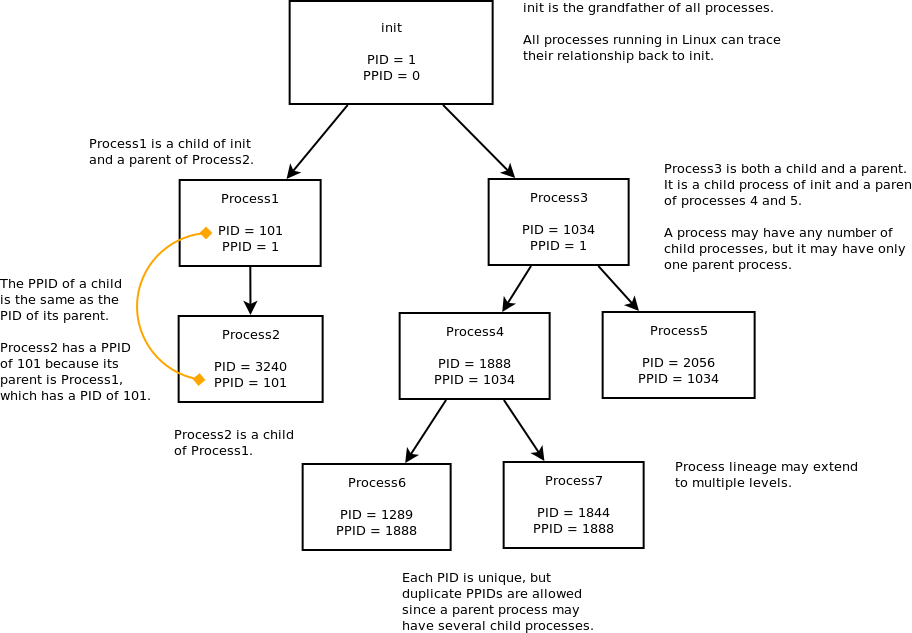
\includegraphics[height=7.5cm]{img/pid_tree.png}
    \caption{An example process tree with init as the parent \cite{webdelight}.}
\end{figure}

Thus, you can think of the processes on a Linux
system as arranged in a \textit{tree}, with the \texttt{init} process at its root.The parent process ID, or \texttt{ppid}, is simply the process ID of the process’s parent.
When referring to process IDs in a C or C++ program, always use the \texttt{pid\_t
typedef}, which is defined in \texttt{<sys/types.h>}. A program can obtain the process ID of
the process it’s running in with the \texttt{getpid()} system call, and it can obtain the process
ID of its parent process with the \texttt{getppid()} system call.

\lstinputlisting[language=c,caption={Get process and parent ID on Linux (\detokenize{src/get_pid.c)}.}, label=src:mylabel]{src/get_pid.c}
If we run the program multiple times under the same shell, the with the \texttt{pid}  will change but the \texttt{ppid} will remain the same as it will be the shell's (parent) \texttt{pid}.

Processing in Linux can be viewed during using the \texttt{ps} command and killed using the \texttt{kill} or \texttt{killall}. See manual for more details.





\subsection{The \texttt{fork} and \texttt{exec} method}

The preferred method to create process in Unix is the \texttt{fork} and \texttt{exec}. This method takes more than one step. \texttt{fork} makes a child process that is \textit{almost} an exact copy of its parent. The new process gets a different PID and has as its PPID the PID of the process that created it.

Because the two processes are now running exactly the same code, they can tell which is which by the return code of fork - the child gets 0, the parent gets the PID of the child. \marginnote{Child and parent are distinguished by the return value of \texttt{fork()}.}  Then using one of the \texttt{exec} family calls, the current process it replaced with a new program. \texttt{exec} loads the program into the current process space and runs it from the entry point \cite{stflowforkexec}.

The two calls are not required to be used together. It's perfectly acceptable for a program to fork itself without execing if, for example, the program contains both parent and child code \cite{stflowforkexec}.




\subsection{The fork() system call}

% see https://www.geeksforgeeks.org/wait-system-call-c/
% see https://www.geeksforgeeks.org/difference-fork-exec/
Fork system call creates a new process, called \emphasis{child process}, which is a copy of the current process (except of their return values) and runs \textit{concurrently} with it. \marginnote{\texttt{fork()} ``returns twice''} The program starts running concurrently at the code location where fork was called. The parent process waits for the child to finish and then resumes.
\begin{figure}[H]
    \centering
    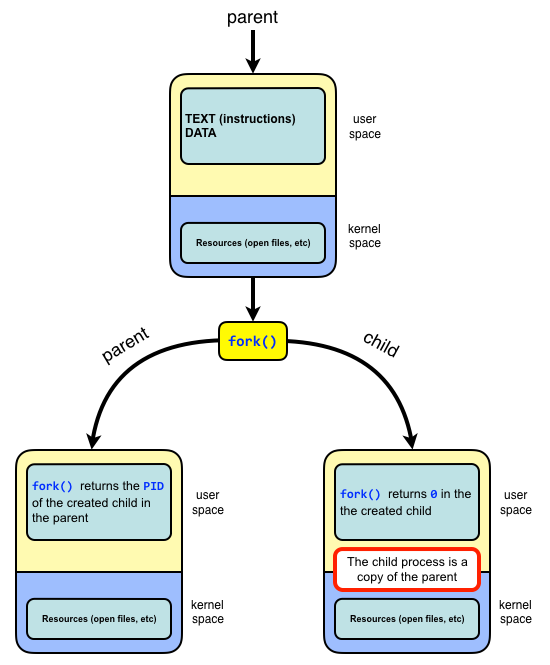
\includegraphics[height=12cm]{img/fork_details.png}
    \caption{How fork works in user space and kernel space.}
\end{figure}

The following diagram illustrates the typical fork/exec operation where the bash shell is used to list a directory with the ls command \cite{stflowforkexec}:
\newpage
\begin{verbatim}
+--------+
| pid=7  |
| ppid=4 |
| bash   |
+--------+
    |
    | calls fork
    V
+--------+             +--------+
| pid=7  |    forks    | pid=22 |
| ppid=4 | ----------> | ppid=7 |
| bash   |             | bash   |
+--------+             +--------+
    |                      |
    | waits for pid 22     | calls exec to run ls
    |                      V
    |                  +--------+
    |                  | pid=22 |
    |                  | ppid=7 |
    |                  | ls     |
    V                  +--------+
+--------+                 |
| pid=7  |                 | exits
| ppid=4 | <---------------+
| bash   |
+--------+
    |
    | continues
    V
\end{verbatim}


\subsection{\texttt{fork()} code and example}
The fork system call does not take an argument. As previously mentioned, the process that invokes the \texttt{fork()} is known as the \textit{parent} and the new process is called the \textit{child}. It returns an integer.
\begin{verbatim}
#include <sys/types.h>
#include <unistd.h>
pid_t fork(void);
\end{verbatim}
\marginnote{Fork's return indicates failure or not.}To differentiate whether its called for the parent or child, it returns different values for each, particularly \cite{webg4gfork}:
\begin{enumerate}
    \item \texttt{fork\_return == -1}: \texttt{fork()} failed and there is no child.
    \item \texttt{fork\_return == 0} returned to the newly created child process.
    \item \texttt{fork\_return > 0}: returned to parent or caller. The value contains process ID of newly created child process
\end{enumerate}

\begin{exmp}
Predict the output of the following snippet of code. \textup{
\lstinputlisting[language=c,caption={How process IDs are assigned to child and parent (\detokenize{src/fork_child_parent.c)}.}, label={src:fork-child-parent}]{src/fork_child_parent.c}
} % textup
\end{exmp}
The output is:
\begin{verbatim}
The main program process ID is 5000
This is the parent process,  with id 5000
The child's process ID is 5001
This is the child process,  with ID 5001
\end{verbatim}

\subsection{(Optional) More fork() examples}

Predict the output of the following examples.
\begin{exmp}
\textup{
\lstinputlisting[language=c,caption={Forked hello world (\detokenize{src/fork_hello.c)}.}, label=src:mylabel]{src/fork_hello.c}
}
\end{exmp}
\begin{verbatim}
Hello world!
Bye world!
Bye world!
\end{verbatim}

\begin{exmp} \textup{\cite{webg4gfork}}
\textup{
\lstinputlisting[language=c,caption={Forked hello world multiple times (\detokenize{src/fork_hellox3.c)}.}, label=src:mylabel]{src/fork_hellox3.c}
} % textup
\end{exmp}
\begin{verbatim}
Hello world!
Hello world!
Hello world!
Hello world!
Hello world!
Hello world!
Hello world!
Hello world!
\end{verbatim}


\begin{exmp}
In this example, although the virtual address of fork() is the same for the parent and child, it maps to different physical addresses therefore parent and child hold different ``instances'' of the variable \texttt{x}.
\textup{
\lstinputlisting[label={src:fork_virt_address},language=c,caption={Accessing the same variable with two processes (\detokenize{src/fork_values2.c)}.}]{src/fork_values2.c}
} % textup
\end{exmp}
\begin{verbatim}
Initially, x = 1 at address 0xa7d99060
Parent has x = 0 at 0xa7d99060
Child has x = 2 at 0xa7d99060
\end{verbatim}


\begin{exmp}
\textup{
\lstinputlisting[language=c,caption={Forked condition (\detokenize{src/fork_tree.c)}.}, label=src:mylabel]{src/fork_tree.c}
} % textup
\end{exmp}

Fig. \ref{fig:fork_tree_sol} illustrates the execution flow. The first \texttt{fork()} in the if statement creates one parent (return value positive) and a child (return 0). For the parent, the OR is true, so it directly enters the block, where it forks again. The child needs to evaluate the second fork and enters the block only for the parent as only the parent satisfies the OR. The final printed output is
\begin{verbatim}
1 1 1 1 1
\end{verbatim}
\begin{figure}[H]
    \centering
    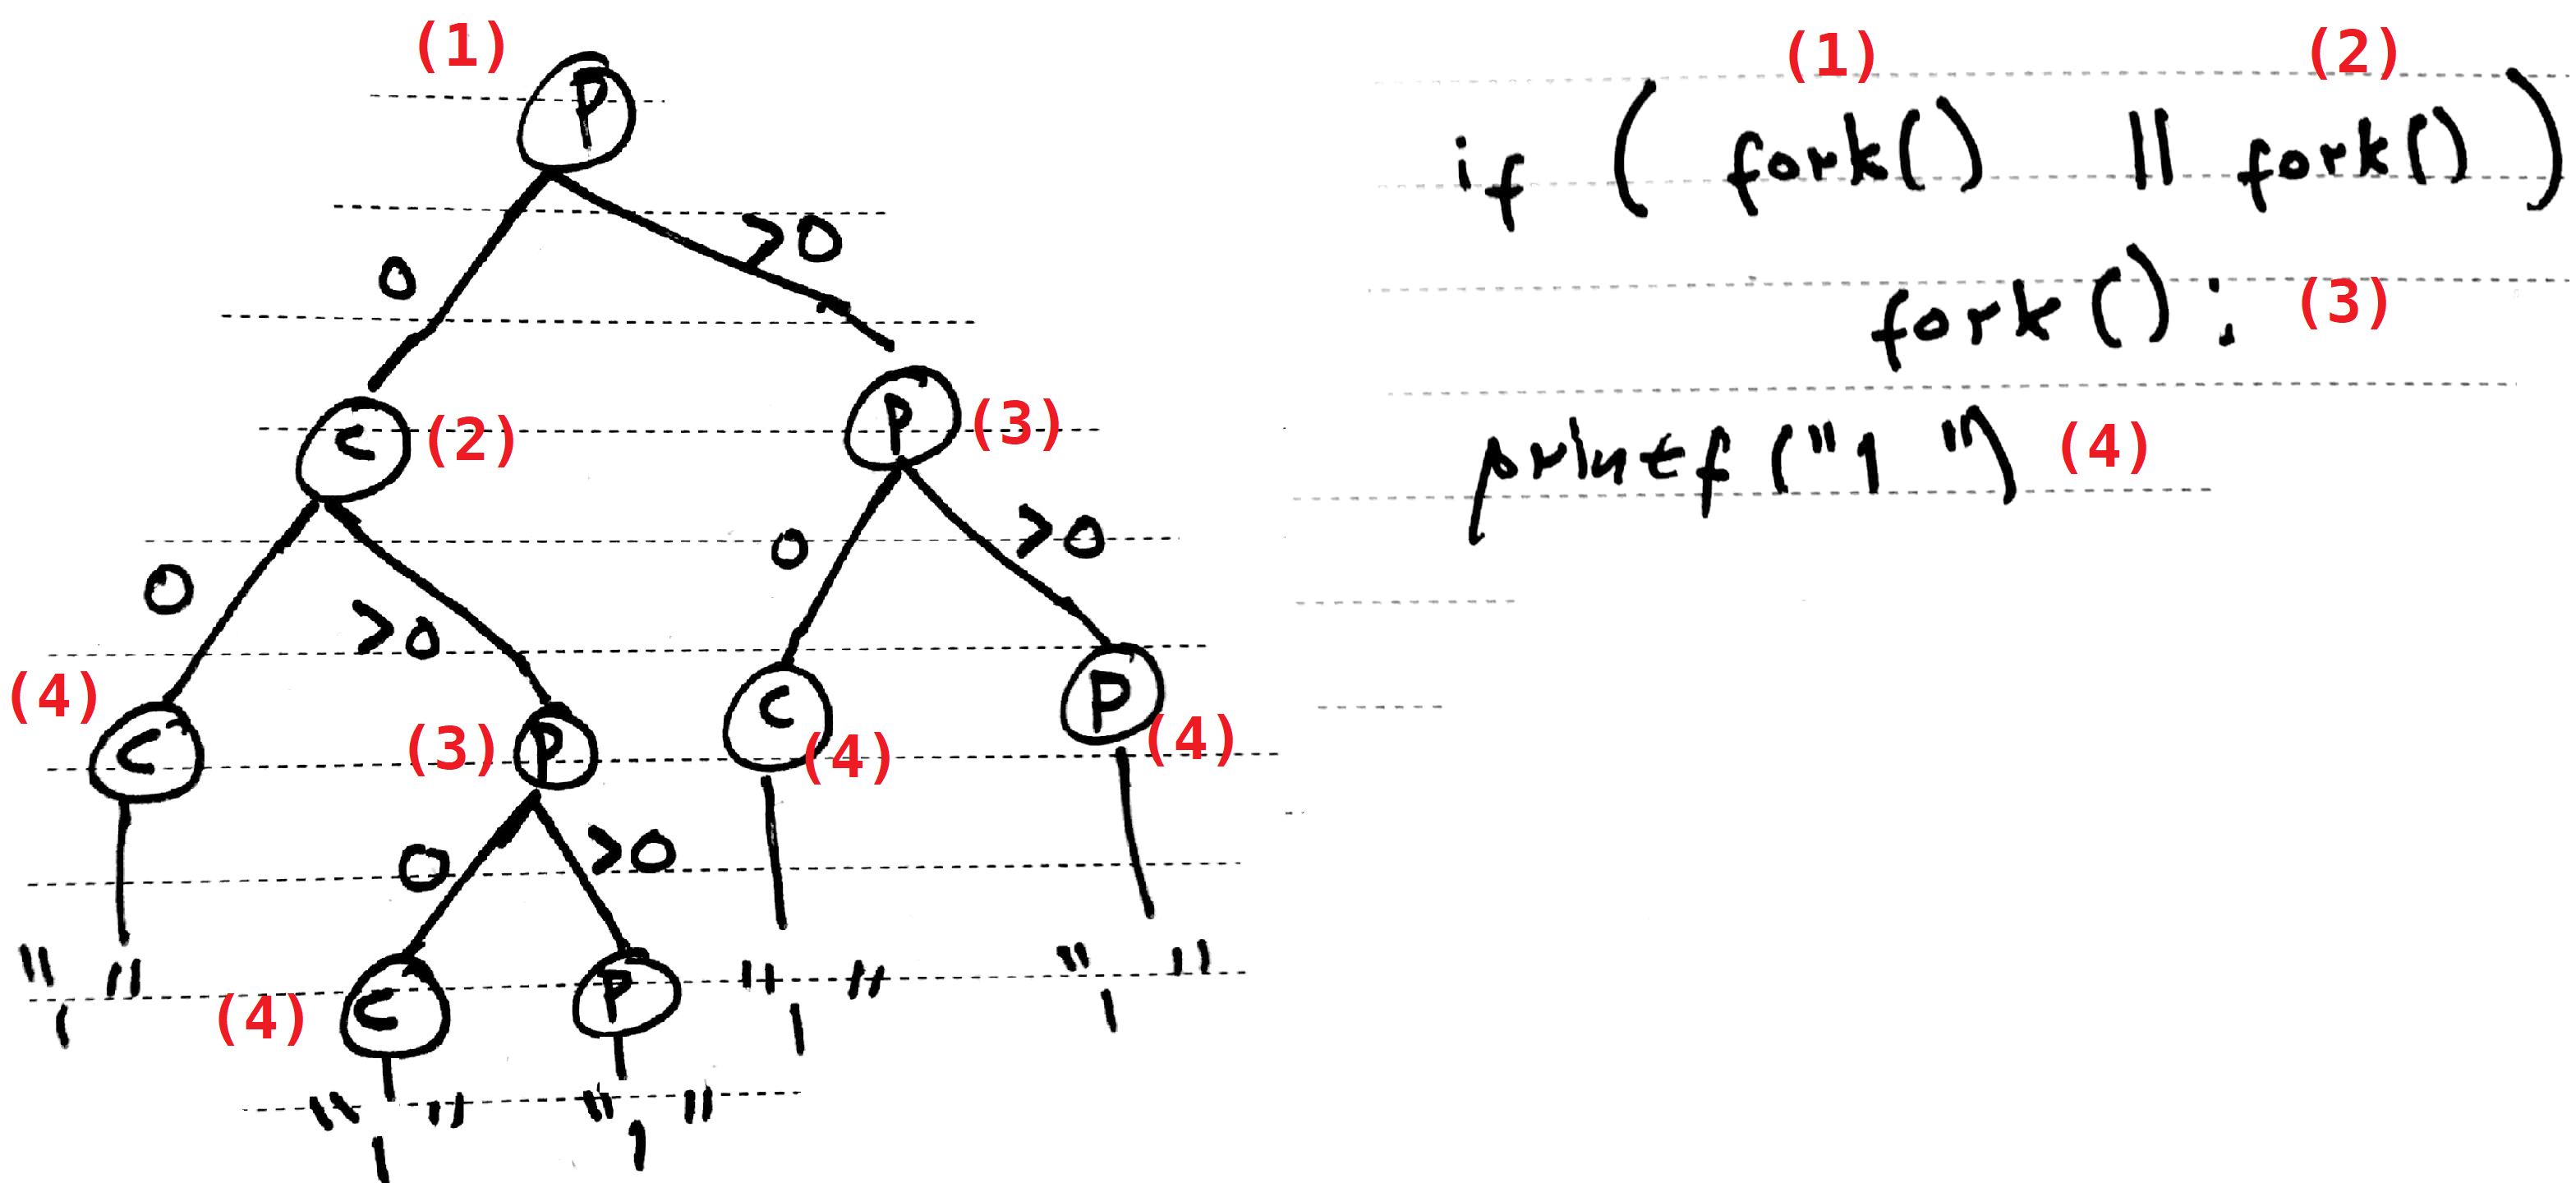
\includegraphics[height=5.25cm]{img/fork_tree_sol.png}
    \caption{Solution to forked condition.}
    \label{fig:fork_tree_sol}
\end{figure}




\section{Executing a process -- the \texttt{exec()} call}


\subsection{The \texttt{exec()} family}
The exec functions replace the program running in a process with another program.
When a program calls an exec function, that process immediately ceases executing that
program and begins executing a new program from the beginning, assuming that the
exec call doesn't encounter an error \cite{bookmitchell}.

There are several variations of the exec function. The name base is exec followed by one of the following letters.
% see https://www.geeksforgeeks.org/exec-family-of-functions-in-c/
% se http://www.it.uu.se/education/course/homepage/os/vt18/module-2/exec/
% see http://openbook.rheinwerk-verlag.de/linux_unix_programmierung/Kap07-009.htm
% see https://ece.uwaterloo.ca/~dwharder/icsrts/Tutorials/fork_exec/
\begin{itemize}
    \item \texttt{int execl ( const char *path, const char *arg, ... );}
    \item \texttt{int execlp( const char *file, const char *arg, ... );}
    \item \texttt{int execle( const char *path, const char *arg, ..., char *const envp[] );}
    \item \texttt{int execv ( const char *path, char *const argv[] );}
    \item \texttt{int execvp( const char *file, char *const argv[] );}
    \item \texttt{int execve( const char *file, char *const argv[], char *const envp[] )}
\end{itemize}
% ref https://ece.uwaterloo.ca/~dwharder/icsrts/Tutorials/fork_exec/
%see https://stackoverflow.com/questions/5769734/what-are-the-different-versions-of-exec-used-for-in-c-and-c
All definitions are found in \texttt{<unistd.h>}. \marginnote{\texttt{exec()} returns (-1) only if it fails.}The \texttt{exec()} functions only return if an error has occurred. The return value is \texttt{-1}, and \texttt{errno} is set to indicate the error. Each system call is the word exec followed by either l or v and then possibly followed by either e or p. If exec is followed by
\begin{itemize}
    \item \texttt{l} , then it expects the arguments as a NULL-terminated \textit{list}, e.g. \texttt{path, arg0, arg1, ..., argn}. The first argument (\texttt{path} or \texttt{file}) describes the program path or file (depending on the p option). \marginnote{\texttt{l}: list} The second, \texttt{arg0} described how the newly spawned process should be named. For example, if \texttt{path = "/bin/ls"}, it would make sense to have \texttt{arg0 = "ls"} but we could also set \texttt{arg0 = "potato"}. \text{arg1, arg2, ..., argm} are in the form of pointers to \texttt{char}. They are the command line options to the program, e.g. in this case they could be \text{"-l", "/"}. The last argument must always be \texttt{NULL} (\texttt{(char* ) 0}). 
    \item \texttt{v}, it is similar but expects the arguments as an \textit{array} of \texttt{char*} (vector). Again, the first argument is the path to the program to execute or the file (depending on the p option) and the second the array of \texttt{char*}. \marginnote{\texttt{v}: vector} In this case, if we wanted to execute the same \texttt{ls -l /} command, we would pass \texttt{\{"/bin/ls", "ls", "-l", "/", NULL\}} to \texttt{execv}.
\end{itemize}
If it is further followed by
\begin{itemize}
    % ref http://vitaly_filatov.tripod.com/ng/tc/tc_000.64.html
    \item \texttt{e}, then it expects  \texttt{char* envp} after the NULL-terminated arguments to the program. \texttt{envp} points to an array of pointers that in turn point to strings
    that define environment variables. \marginnote{\texttt{e}: environ
    ment} These strings usually have the form:  \texttt{ENVVAR=value} where \texttt{ENVVAR} is the name of the environment
    variable and \texttt{value} is the string value to set it to.  The \texttt{envp} array is \textit{also} terminated by a NULL pointer.  If \texttt{envp} is NULL, then the
    child process acquires the environment of the calling process. For example, we could have
    % ref http://openbook.rheinwerk-verlag.de/linux_unix_programmierung/Kap07-009.htm
    \begin{verbatim}
    char * environment [4];
    environment [0]="SHELL=/bin/csh";
    environment [1]="LOGNAME=heino";
    environment [2]="OSTYPE=LiNuX";
    environment [3]=NULL;
    \end{verbatim}
    % ref https://stackoverflow.com/questions/21558937/i-do-not-understand-how-execlp-works-in-linux9
    \item \texttt{p}, it will search for the file using the current environment \marginnote{\texttt{p}: PATH} variable PATH, which usually includes /bin/, /usr/bin/, etc.
\end{itemize}
Their differences are summarised in the table below.
\begin{figure}[H]
    % ref https://zodml.org/sites/default/files/Advanced_Programming_in_the_UNIX_Environment%2C_3rd_Edition.pdf p288
    \centering
    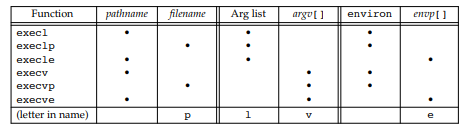
\includegraphics[height=3cm]{img/exec_family_table.png}
    \caption{The 6 exec functions}
\end{figure}

\subsection{\texttt{exec} basic examples}


Some basic examples that show the usage of  the exec family are listed below.
% see also https://zodml.org/sites/default/files/Advanced_Programming_in_the_UNIX_Environment%2C_3rd_Edition.pdf p288


%%% table of code
\lstset{
  language=C,
  basicstyle=\small,
  breaklines=true,
  backgroundcolor=\color{white}
 }

\begin{tabular}{0.5\textwidth|0.5\textwidth}
\textbf{execl.c } &  \textbf{execv.c}\\
\begin{lstlisting}
#include <unistd.h>    // exec*

int main () {
	/* Executes ls -l / */
	char* cmd = "/bin/ls";// executable
	char* argv0 = "ls";   // name to use
	char* argv1 = "-l";   // cmd arg
	char* argv2 = "/";    // cmd arg
	char* argv3 = NULL;   // terminator

	return execl (cmd, argv0,  argv1,
	argv2, NULL);
}
\end{lstlisting}&

\begin{lstlisting}
#include <unistd.h>    // exec*

int main () {
	/* Executes ls -l / */
	char* cmd = "/bin/ls";
	char* argv[4];
	argv[0] = "ls";
	argv[1] = "-l";
	argv[2] = "/";
	argv[3] = NULL;

	return execv(cmd,  argv);
}
\end{lstlisting}\\

\textbf{execlp.c} & \textbf{execvp.c} \\
\begin{lstlisting}
#include <unistd.h>    // exec*

int main () {
	/* Executes ls -l / */
	char* cmd = "ls";     // executable
	char* argv0 = "ls";   // name to use
	char* argv1 = "-l";   // cmd arg
	char* argv2 = "/";    // cmd arg
	char* argv3 = NULL;   // terminator

	return execlp (cmd, argv0,  argv1,
	argv2, NULL);
}
\end{lstlisting}&
\begin{lstlisting}
#include <unistd.h>    // exec*

int main () {
	/* Executes ls -l / */
	char* cmd = "ls";
	char* argv[4];
	argv[0] = "ls";
	argv[1] = "-l";
	argv[2] = "/";
	argv[3] = NULL;

	return execvp (cmd,  argv);
}
\end{lstlisting}\\

\textbf{execle.c} & \textbf{execve.c }\\
\begin{lstlisting}
#include <unistd.h>
#include <stdio.h>

int main() {
	/* Executes env given some arguments
	in  envp */
	char* fpath = "/bin/sh";
    char* arg[] = { fpath, "-c", "env",
                    NULL };
    char* envp[] =
    {
        "HOME=/",
        "PATH=/bin:/usr/bin",
		"USER=leo", 
		"TERM=xterm", 
		NULL
    };
    execle(fpath, arg[0], arg[1], 
        arg[2], NULL, envp);
    fprintf(stderr, "Oops!\n");
    return -1;
}

\end{lstlisting}&
\begin{lstlisting}
#include <unistd.h>
#include <stdio.h>

int main() {
	/* Executes env given some arguments   
	in  envp */
	char* fpath = "/bin/sh";
    char* arg[] = { fpath, "-c", "env", 
                    NULL };
    char* envp[] =
    {
        "HOME=/",
        "PATH=/bin:/usr/bin",
		"USER=leo", 
		"TERM=xterm", 
       	NULL 
    };
    execve(fpath, arg, envp);
    fprintf(stderr, "Oops!\n");
    return -1;
}

\end{lstlisting}\\
\end{tabular} 
%%% table of code end
%%% code listings
\lstdefinestyle{code1}{
    backgroundcolor=\color{lightestestpink},   
    commentstyle=\color{codegrayblue},
    keywordstyle=\color{DarkerPink},
    numberstyle=\tiny\color{codegray},
    stringstyle=\color{black!40!cyan},
    basicstyle=\small\ttfamily,
    breakatwhitespace=false,
    breaklines=true,        
    captionpos=t,             
    keepspaces=true,        
    numbers=left,           
    numbersep=5pt,
    showspaces=false, 
    showstringspaces=false,
    showtabs=false,
    tabsize=4
}
\lstset{style=code1}

In the \texttt{exece} examples, we do not expect to hit the ``Oops!'' message as the program image will be replace with the one called by \texttt{exece} unless an error occurs. Also, the system will append some additional environment variables to the defined ones, so the output looks something like:
\begin{verbatim}
PWD=/tmp
HOME=/
TERM=xterm
USER=leo
SHLVL=0
PATH=/bin:/usr/bin
_=/bin/env
\end{verbatim}


\subsection{A commot \texttt{exec} pitfall}

The bug below demonstrates why it's always good to check if \texttt{exec} executed without errors.
\begin{exmp}
What's wrong with this code?
% ref https://github.com/angrave/SystemProgramming/wiki/Process-Control%2C-Part-1%3A-Wait-macros%2C-using-signals
\textup{
\lstinputlisting[language=c,caption={How many processes are created? (\detokenize{src/exec_fork_bug.c)}.}, ]{src/exec_fork_bug.c}
} % textup
\end{exmp}
\marginnote{It's a good practice to \texttt{exit} after \texttt{exec} in case it fails.}We misspelled \texttt{ehco}, so we can't \texttt{exec} it. The first time, instead of being replaced with another program, the child will continue and get forked in 2. Then the two children will do the same and get forked in $4,\ldots, ... 2^{10}$ processes, ``fork bombing'' our machine. How could we prevent this? Put an \texttt{exit} (\texttt{exit(int status)} right after \texttt{exec} so in case \texttt{exec} fails we won't end up fork bombing our machine.



\subsection{The \texttt{fork-exec} pattern}

A common pattern to run a subprogram within a program is first to fork the process
and then exec the subprogram. This allows the calling program to continue execution
in the parent process while the calling program is replaced by the subprogram in the child process

The code below demonstrates how to replace the child with another program which runs the \texttt{ls -l /} command.



\lstinputlisting[label={src:fork-exec},language=c,caption={Using fork followed by exec (\detokenize{src/fork-exec.c)}.}, ]{src/fork-exec.c}

The output of this looks something like:
\begin{verbatim}
done with main program
total 52
lrwxrwxrwx   1 root root     7 Dec  6  2018 bin -> usr/bin
drwxr-xr-x   3 root root  4096 Apr  4 22:30 boot
drwxr-xr-x  21 root root  3580 Jun  5 17:53 dev
<-- omitted -->
\end{verbatim}
Notice that the output of ls (child) appears \textit{after} the parent has terminated.

% see https://github.com/angrave/SystemProgramming/wiki/Forking,-Part-2:-Fork,-Exec,-Wait
% see https://www.softprayog.in/programming/creating-processes-with-fork-and-exec-in-linux


\section{Controlling processes with signals}

\textbf{NOTE}: Before reading this chapter, remember that signal handlers should do as little as they can and operations should be atomic (1 cycle). The code used is only for API demonstration purposes and should not be used in practice.  Signal handlers should also not print anything.
% see https://www.geeksforgeeks.org/signals-c-language/
% https://www.thegeekstuff.com/2012/03/catch-signals-sample-c-code/
% https://gist.github.com/aspyct/3462238
% see https://www.systutorials.com/5510/catching-the-signal-sent-by-kill-in-c-on-linux/
% https://www.geeksforgeeks.org/signals-c-language/
% https://www.thegeekstuff.com/2012/03/catch-signals-sample-c-code/
% https://www.ibm.com/support/knowledgecenter/en/ssw_ibm_i_72/apis/sigkill.htm
% https://renenyffenegger.ch/notes/Linux/kernel/process/signal
% https://gist.github.com/aspyct/3462238
% https://github.com/angrave/SystemProgramming/wiki/Process-Control%2C-Part-1%3A-Wait-macros%2C-using-signals#signals
% https://zodml.org/sites/default/files/Advanced_Programming_in_the_UNIX_Environment%2C_3rd_Edition.pdf 313/347


\subsection{What are Unix signals?}
% ref https://www.bogotobogo.com/Linux/linux_process_and_signals.php
% https://zodml.org/sites/default/files/Advanced_Programming_in_the_UNIX_Environment%2C_3rd_Edition.pdf 347
\begin{definition}
\emphasis{Signal} is a notification, a message sent by either operating system or some application to our program. Signals are a software interrupt mechanism for one-way asynchronous notifications. A signal may be sent from the kernel to a process, from a process to another process, or from a process to itself.
\end{definition}
Linux kernel $\geq 3.2.0$ implements 31 signals (\url{http://poincare.matf.bg.ac.rs/~ivana/courses/ps/sistemi_knjige/pomocno/apue/APUE/0201433079/ch10lev1sec2.html#ch10fig01}). Every signal has a name starting from the characters  \texttt{SIG}. Signals don't carry any argument and their names are mostly self explanatory. For example, \texttt{SIGABRT} is the abort signal that is generated when a process calls the \texttt{abort}
function. Signal names are all defined by positive integer constants (the signal number) in the
header \texttt{<signal.h>}. Each one is identified by a number from 1 to 31. 

We can tell the kernel to do one of three things when a signal occurs. We call this the \emphasis{disposition} of the signal, or the action associated with a signal.

% ref https://zodml.org/sites/default/files/Advanced_Programming_in_the_UNIX_Environment%2C_3rd_Edition.pdf 347
\begin{enumerate}
    \item \textit{Ignore} the signal. This works for most signals, but two signals can never be
ignored: SIGKILL and SIGSTOP.
    \item \textit{Catch} (handle) the signal.To do this, we tell the kernel to call a function of ours
whenever the signal occurs. For example, if
the process has created temporary files, we may want to write a signal-catching
function for the \texttt{SIGTERM} signal (the termination signal that is the default signal
sent by the \texttt{kill} command) to clean up the temporary files.
    \item Let the \textit{default action} apply. Every signal has a default action -- for most signals it is to terminate the
process.
\end{enumerate}



\subsection{Catch signal -- the \texttt{signal} function}
% ref https://zodml.org/sites/default/files/Advanced_Programming_in_the_UNIX_Environment%2C_3rd_Edition.pdf 347
The simplest interface to the signal features of the UNIX System is the signal function.
\begin{verbatim}
#include <signal.h>

typedef void (*sighandler_t)(int);
sighandler_t signal(int signum, sighandler_t handler);
// Returns: previous disposition of signal if OK, SIG_ERR on error
\end{verbatim}
% ref https://www.tutorialspoint.com/c_standard_library/c_function_signal.htm
\begin{itemize}
    \item \texttt{sig} -- This is the signal number (from 1 to 31) to which a handling function is set. All signal numbers are explained in table \TODO and declared in \texttt{signal.h}. 
    \item func -- This is a pointer to a function. This can be a function defined by the programmer or one of the following predefined functions:
    \begin{enumerate}
        \item \texttt{SIG\_DFL} -- Default handling. The signal is handled by the default action for that particular signal.
        \item \texttt{SIG\_IGN} -- Ignore Signal. The signal is ignored.
    \end{enumerate}
    \item \texttt{return} -- returns the previous value of the signal handler, or \texttt{SIG\_ERR} on error.
\end{itemize}

\begin{exmp}

This example demonstrates how to catch a \texttt{SIGINT} signal. \texttt{SIGINT} is generated e.g. when the user presses \texttt{Ctr-C}.
% ref https://www.tutorialspoint.com/c_standard_library/c_function_signal.htm
\textup{
\lstinputlisting[label={src:signal-catch},language=c,caption={Catching and handling a \texttt{SIGINT} using the \texttt{signal} function (\detokenize{src/signal_catch.c)}.}, ]{src/signal_catch.c}
} % textup
\end{exmp}
After waiting for a few seconds and pressing \texttt{Ctr-C}, the output is the following.
\begin{verbatim}
Going to sleep for a second...
Going to sleep for a second...
Going to sleep for a second...
Going to sleep for a second...
^CCaught signal 2, coming out...

shell returned 1
\end{verbatim}


\subsubsection{User-defined signals}

Linux also provides two user-defined signals, namely \texttt{SIGUSR1} and \texttt{SIGUSR2}. \texttt{SIGUSR1} for instance can be emitted from the terminal with the \texttt{kill} command:
\begin{verbatim}
$ kill -USR1 PID_NUMBER
\end{verbatim}
%%% see ex,m https://zodml.org/sites/default/files/Advanced_Programming_in_the_UNIX_Environment%2C_3rd_Edition.pdf 358
\begin{exmp}

This example demonstrates how to catch \texttt{SIGUSR} signals. Note that the  \texttt{pause} function simply suspends the calling process until a signal is received.

\textup{
\lstinputlisting[language=c,caption={Handling user signal (\detokenize{src/signal_user.c)}.}, ]{src/signal_user.c}
}
\end{exmp}
If we run this program, note its PID:
\begin{verbatim}
my PID is 1557, send signal
\end{verbatim}
Then open another terminal and type
\begin{verbatim}
$ kill -USR1 1557
$ kill -USR2 1557
$ kill 1557
\end{verbatim}
then the output is
\begin{verbatim}
received SIGUSR1
received SIGUSR2
Terminated
\end{verbatim}
Note that by default \texttt{kill} sends \texttt{SIGTERM}.




\subsection{Send signal -- the \texttt{kill} function}




% ref https://www.ibm.com/support/knowledgecenter/en/ssw_ibm_i_72/apis/sigkill.htm
The kill() function sends a signal to a process or process group specified by pid. The signal to be sent is specified by sig and is either 0 or one of the signals from the list in the <sys/signal.h> header file.

The process sending the signal must have appropriate authority to the receiving process or processes. The kill() function is successful if the process has permission to send the signal sig to any of the processes specified by pid. If kill() is not successful, no signal is sent.
\begin{verbatim}
#include <signal.h>

int kill(pid_t pid, int sig);
\end{verbatim}





% see https://pubs.opengroup.org/onlinepubs/009695399/functions/kill.html
The \texttt{kill()} function shall send a signal to a process or a group of processes specified by pid. The signal to be sent is specified by \texttt{sig} and is either one from the list given in \texttt{<signal.h>} or 0. If \texttt{sig} is 0 (the null signal), error checking is performed but no signal is actually sent. The null signal can be used to check the validity of pid.

If \texttt{pid} is
\begin{itemize}
    \item $>0$, \texttt{sig} shall be sent to the process whose process ID is equal to pid.
    \item $0$, \texttt{sig} shall be sent to all processes (excluding an unspecified set of system processes) whose process group ID is equal to the process group ID of the sender, and for which the process has permission to send a signal.
    \item $-1$, \texttt{sig} shall be sent to all processes (excluding an unspecified set of system processes) for which the process has permission to send that signal.
\end{itemize}
\texttt{int sig}:
As already mentioned, \texttt{sig} is the signal number to send with value from 1 to 31 for modern Linux kernels, defined in \texttt{<signal.h>}. 

\texttt{return}: Upon successful completion, \texttt{0} shall be returned. Otherwise, \texttt{-1} shall be returned and \texttt{errno} set to indicate the error.

Below are some typical \texttt{kill()} examples to control the child.
% ref https://github.com/angrave/SystemProgramming/wiki/Process-Control%2C-Part-1%3A-Wait-macros%2C-using-signals#how-do-i-killstopsuspend-my-child-from-c
\begin{verbatim}
kill(child, SIGUSR1); // Send a user-defined signal
kill(child, SIGSTOP); // Stop the child process (the child cannot prevent this)
kill(child, SIGTERM); // Terminate the child process (the child can prevent this)
kill(child, SIGINT); // Equivalent to CTRL-C (by default closes the process)
\end{verbatim}



\subsubsection{\texttt{kill()} examples}
%%% see
% https://github.com/angrave/SystemProgramming/wiki/Process-Control%2C-Part-1%3A-Wait-macros%2C-using-signals#signals
% https://www.geeksforgeeks.org/signals-c-language/
% https://www.cs.cmu.edu/afs/cs/academic/class/15213-f11/www/code/14-signals/forks.c
%%%
\begin{exmp}
The listing below demonstrates how a process can send SIGINT to itself, terminating itself.
\end{exmp}
\lstinputlisting[language=c,caption={A process sending SIGINT to itself (\detokenize{src/kill_suicide.c)}.}, label=src:mylabel]{src/kill_suicide.c}




\section{Waiting for process termination}


\subsection{Why wait for children to complete?}

Going back to fork-exec, if we run the code in Listing \ref{src:fork-exec}, it is not certain whether the child or parent will finish first and in general, this cannot be predicted when we use the fork-exec model. That’s because the child process, in which ls is run, is scheduled independently of the parent process.

In some situations, though, it is desirable for the parent process to wait until one or
more child processes have completed.This can be done with the wait family of system
calls. \marginnote{Why use the wait functions?}These functions allow you to wait for a process to finish executing, and enable
the parent process to retrieve information about its child’s termination.

% signals more: https://www.linuxjournal.com/article/3985,
% https://www.usna.edu/Users/cs/aviv/classes/ic221/s16/lec/19/lec.html
Another reason why wait should be used by the parent is because When a process ends via \texttt{exit} or \texttt{return}, all of the memory and resources associated with it are deallocated so they can be used by other processes. However, the process's entry in the process table remains. When a process terminates, the kernel asynchronously sends a SIGCHLD \emphasis{signal} (software interrupt) to the parent. The parent can read the child's exit status by executing the wait system call, which reads the SIGCHLD signal. Parent, on receipt of SIGCHLD reaps the status of the child from the process table.

% see https://books.google.de/books?id=aOh1DwAAQBAJ&pg=PA369&lpg=PA369&dq=linux+why+does+parent+have+to+wait+for+children&source=bl&ots=s1gnbguML1&sig=ACfU3U2Xhcdebz4wznuLMNZsu11eJyPdvA&hl=en&sa=X&ved=2ahUKEwjmtqHgh-HiAhWGL1AKHZzsDLk4ChDoATABegQIBBAB#v=onepage&q=linux%20why%20does%20parent%20have%20to%20wait%20for%20children&f=false
When we use the fork-exec model and a child process runs, Unix allocates it memory (for opened files etc.) and a PID in the process table. When the child terminates, the system flushes and closes all opened files and data structures and sends an asynchronous SIGCHLD signal to the parent but does not remove the child's PID entry from the process table. Without using wait(), the parent fails to catch the SIGCHLD hence does not remove the terminated child's PID from the process table. That PID corresponds to a dead process (\emphasis{zombie process}). In the shell, zombie processes can be listed with the \texttt{ps Z} command.

Zombie processes shouldn't exist because the amount of kernel memory although they take insignificant memory, they reserve (dead) PID entries. A way to kill a zombie process is by killing its parent. 

On the other hand, if the parent terminates while its children are running, then its "zombie" children (if any) are adopted by init. init automatically performs a wait to remove the zombies. This type of zombie processes are called \emphasis{orphans}.

The figure below shows how a healthy fork-exec-wait cycle should look like.
\begin{figure}[H]
    \centering
    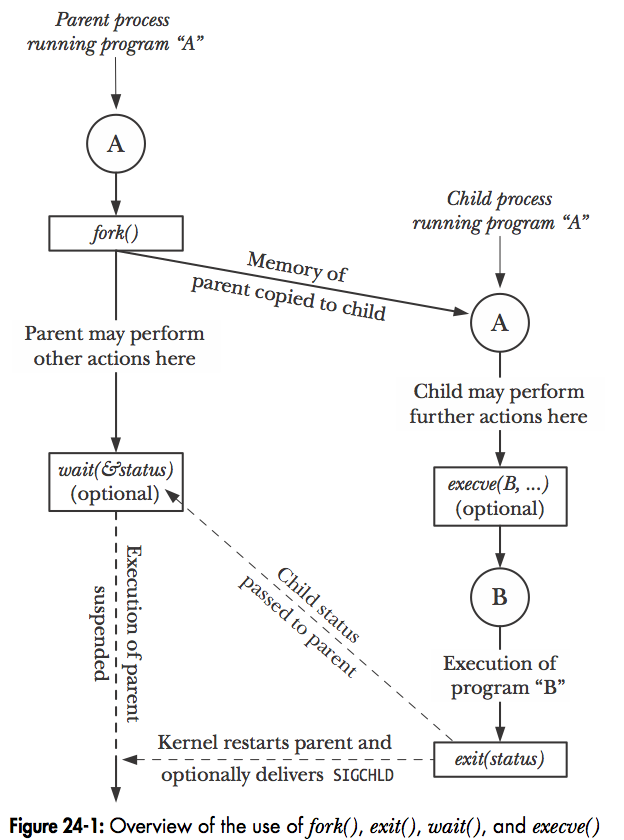
\includegraphics[height=9.5cm]{img/fork-exec-wait cycle.png}
    \caption{fork-exec-wait model overview.}
\end{figure}



\subsection{Creating and observing a zombie process}

In Listing \ref{src:fork-child-parent}, the parent doesn't call \texttt{wait}. As a result, a zombie child process is created for a breif amount of time from the moment the child terminates till the parent returns. To observe, add the header
\begin{verbatim}
#include <wait.h>
\end{verbatim}
add the line
\begin{verbatim}
sleep(100);
\end{verbatim}
after the if-else statement. Then for the next 100 seconds, a zombie will be created. Run the program and in another terminal get the child's PID:
\begin{verbatim}
<-- omitted -->
This is the child process,  with ID 8630
\end{verbatim}
Run \texttt{ps Z} in another terminal to list the zombie processes and 8630 should be in them:
\begin{verbatim}
-                                8630 pts/0    S+     0:00 ./a.out
\end{verbatim}



\subsection{The \texttt{wait()} system call}
% https://www.usna.edu/Users/cs/aviv/classes/ic221/s16/lec/14/lec.html
The \texttt{wait()} system call is used by a parent process to wait for the status of the child to change. wait() suspends the execution of the calling process until one of its child processes exits or a signal is received. A child process may terminate due to any of these:
\begin{itemize}
    \item It calls exit();
    \item It returns (an int) from main
    \item It receives a signal (from the OS or another process) whose default action is to terminate. 
\end{itemize}


\subsubsection{The \texttt{wait} family of functions}
There are the \texttt{wait, waitpid, waitid, wait3, wait4} in the wait family, but we will only concern ourselves with the first two:

% see http://man7.org/linux/man-pages/man2/wait.2.html
% see https://webdocs.cs.ualberta.ca/~tony/C379/C379Labs/Lab3/wait.html
% see http://poincare.matf.bg.ac.rs/~ivana/courses/ps/sistemi_knjige/pomocno/apue/APUE/0201433079/ch08lev1sec6.html
\begin{verbatim}
#include <sys/types.h>
#include <sys/wait.h>

pid_t wait(int *wstatus);
pid_t waitpid(pid_t pid, int *wstatus, int options);
\end{verbatim}
% ref https://www.ibm.com/support/knowledgecenter/en/SSLTBW_2.3.0/com.ibm.zos.v2r3.bpxbd00/rtwaip.htm:
Regarding the arguments, the values they can take are for \texttt{pid\_t pid} \marginnote{\texttt{wait} and \texttt{waitpid} calls}
\begin{itemize}
    \item $<-1$, meaning wait for any child process whose process group ID is equal to the absolute value of pid.
    \item $-1$, meaning wait for any child process.
    \item 0, meaning wait for any child process whose process group ID is
              equal to that of the calling process.
    \item $> 0$, meaning wait for the child whose process ID is equal to the value of pid.
\end{itemize}
\texttt{int *wstatus}:
\begin{itemize}
    \item Points to a location where \texttt{waitpid()} can store a status value. This status value is zero if the child process explicitly returns zero status. Otherwise, it is a value that can be analysed with the certain \textit{status analysis macros} described later.
\end{itemize}
\texttt{int options}:
\begin{itemize}
    \item \texttt{WNOHANG}: Return immediately if no child has exited.
    \item \texttt{WUNTRACED}: Also return if a child has stopped. Status for traced children which have stopped is provided even if this option is not specified.
    \item \texttt{WCONTINUED}: Also return if a stopped child has been resumed by delivery of \texttt{SIGCONT}.
\end{itemize}
%ref https://zodml.org/sites/default/files/Advanced_Programming_in_the_UNIX_Environment%2C_3rd_Edition.pdf 238
\marginnote{If an error had occured after waiting, we know it from the return value}Return value (same for both):
\begin{itemize}
    \item process ID if OK,
    \item if non-blocking option and no zombies around,
    \item or -1 on error.
\end{itemize}
As mentioned before the return status of the child in \texttt{waitpid} is stored in \texttt{int\& wstatus} and does not directly provide useful information but can be analysed with the \texttt{WIF*} macros. The top row shows what the macro means if it evaluates to true and the bottom how its exit code is interpreted.

% see https://www.gnu.org/software/libc/manual/html_node/Process-Completion-Status.html
\begin{enumerate}
    \item \texttt{WIFEXITED(status) == true} then the child exited normally
and \texttt{WEXITSTATUS(status)} is the return code when child exits.
    \item \texttt{WIFSIGNALED(status) == true} then the child exited because a signal was not caught and 
\texttt{WTERMSIG(status)} gives the number of the terminating signal.
    \item \texttt{WIFSTOPPED(status) == true} then the child is stopped and 
\texttt{WSTOPSIG(status)} is gives the number of the stop signal
\end{enumerate}

To summarise, \texttt{waitpid} is more flexible as is allows a process to be made non-blocking via \texttt{options} and can select which child process to wait via \texttt{pid}.




\subsection{Practical examples of the \texttt{wait()} call}


% see also https://github.com/angrave/SystemProgramming/wiki/Process-Control,-Part-1:-Wait-macros,-using-signals


\begin{exmp}
\textup{
\lstinputlisting[language=c,caption={Waiting for child and getting its status (\detokenize{src/fork_exec_wait.c)}.}, label=src:mylabel]{src/fork_exec_wait.c}
}
\end{exmp}
Output:
\begin{verbatim}
total 2080564
drwxr-xr-x   2 root root       4096 Mai 13 11:48 bin
drwxr-xr-x   3 root root       4096 Mai 23 10:06 boot
drwxrwxr-x   2 root root       4096 Aug 30  2018 cdrom
drwxr-xr-x  18 root root       3960 Jun 13 09:06 dev
<-- omitted -->
the child process exited normally, with exit code 0
\end{verbatim}
%------------- end of example ------------- %


\begin{exmp}
\textup{
\lstinputlisting[language=c,caption={Status code of multiple children (\detokenize{src/wait_pid_array.c)}.}, label=src:mylabel]{src/wait_pid_array.c}
}
\end{exmp}
Output:
\begin{verbatim}
Child 5315 terminated with status: 100
Child 5316 terminated with status: 101
Child 5317 terminated with status: 102
Child 5318 terminated with status: 103
Child 5319 terminated with status: 104
\end{verbatim}
%------------- end of example ------------- %


\begin{exmp}
When the parent hits a \texttt{wait()}, it pauses its execution and waits for the other forked branch, the child to finish. Then it continues. Such a flow is demonstrated below.
\textup{
\lstinputlisting[language=c,caption={Waiting to synchronise with child (\detokenize{src/fork_sync.c)}.}, label=src:mylabel]{src/fork_sync.c}
}
\end{exmp}
Output:
\begin{verbatim}
HP: hello from parent
HC: hello from child
Bye
CT: child has terminated
Bye
\end{verbatim}
In this case, when the parent sees the \texttt{wait()}, it pauses its execution and wait's for the child's if branch to finish. The following diagram explains the flow.
% ref https://www.cs.cmu.edu/afs/cs/academic/class/15213-f10/www/lectures/12-exceptions.pdf
\begin{figure}[H]
    \centering
    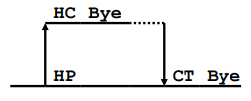
\includegraphics[height=1.75cm]{img/fork_sync_diagram.PNG}
    \caption{Synchronising child and parent in the example.}
\end{figure}
%------------- end of example ------------- %


\begin{exmp}
This example shows a principle similar to the one in Listing \ref{src:fork_virt_address}. Although the child inherits the same virtual address space, the actual physical address of variable \texttt{var} is different between then so each one holds a different instance of the variable.
\textup{
\lstinputlisting[language=c,caption={Modifying the same variable in a child and in a parent using a signal handler (\detokenize{src/sig_wait_val.c)}.}, ]{src/sig_wait_val.c}
}
\end{exmp}
Output:
\begin{verbatim}
[child] val = 7
[parent] val = 15
\end{verbatim}


\subsection{More advanced examples}
% see also: http://condor.depaul.edu/glancast/374class/hw/samplefinal.html

\begin{exmp}
What's the output of the following program?
\textup{
\lstinputlisting[language=c,caption={Fork followed by waiting for  status  (\detokenize{src/fork_waitpid.c)}.}, ]{src/fork_waitpid.c}
} % textup
\end{exmp}
The order of \text{0} (for parent) and \texttt{1} (for child) may change. The diagram below explains the flow.
\begin{figure}[H]
    \centering
    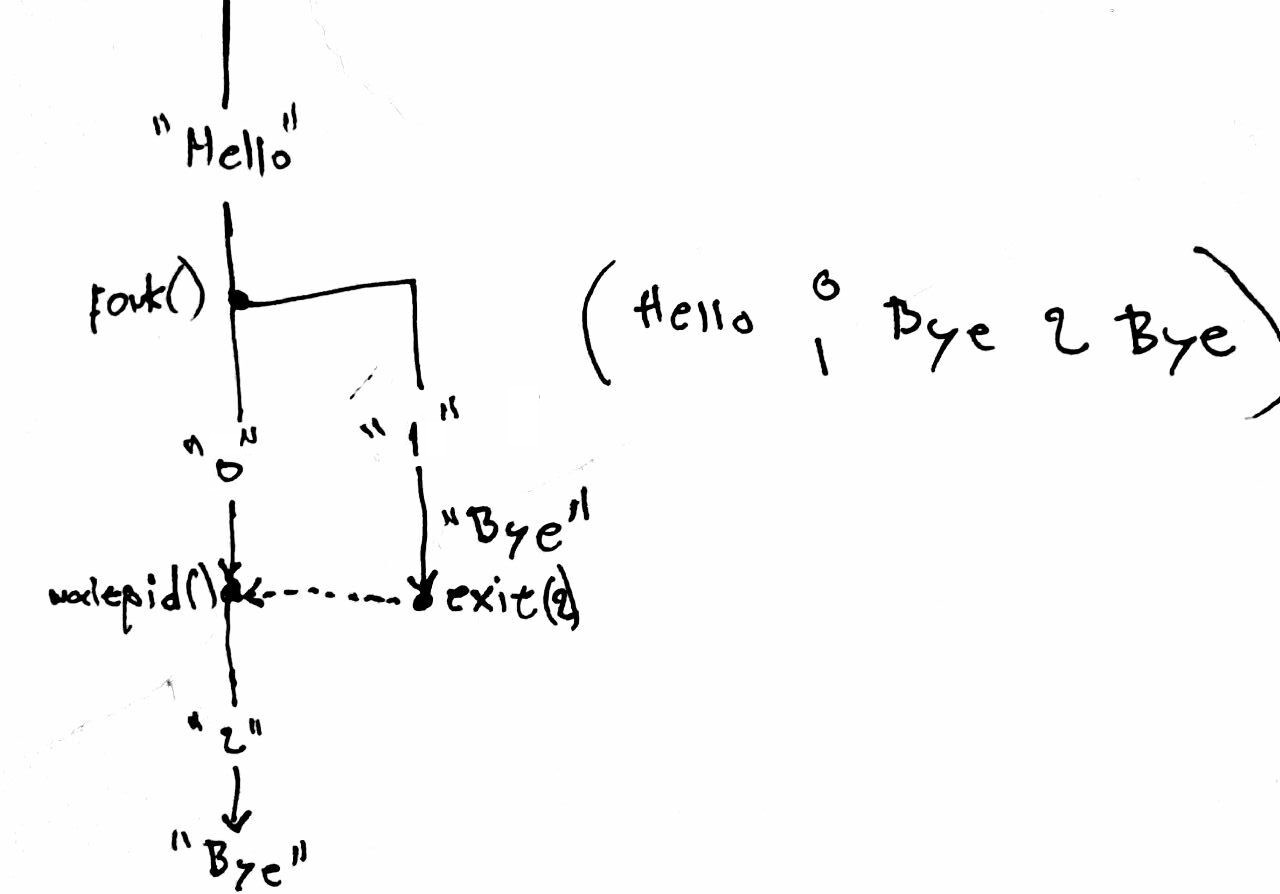
\includegraphics[height=6cm]{img/fork_waitpid_sol.jpg}
    \caption{Flow diagram for the example.}
\end{figure}
\begin{verbatim}
Hello
0
1
Bye
2
Bye

shell returned 2
\end{verbatim}

\begin{exmp}
\textup{
\lstinputlisting[language=c,caption={Forking, killing and waiting for status of multiple children (\detokenize{src/fork_kill_wait.c)}.}, ]{src/fork_kill_wait.c}
} % textup
\end{exmp}
Output:
\begin{verbatim}
Killing process 29280
Killing process 29281
Killing process 29282
Killing process 29283
Killing process 29284
Child 29280 terminated abnormally
Child 29281 terminated abnormally
Child 29282 terminated abnormally
Child 29283 terminated abnormally
Child 29284 terminated abnormally
\end{verbatim}

%------------- end of example ------------- %
\begin{exmp}
This example is almost the same as the previous but additionally includes a signal handler attached to signal \texttt{SIGINT}.
\textup{
\lstinputlisting[language=c,caption={Fork children, send them SIGINT, use a signal handler and wait (\detokenize{src/fork_kill_signal_wait.c)}.}, ]{src/fork_kill_signal_wait.c}
} % textup
\end{exmp}
Output:
\begin{verbatim}
Killing process 1269
Killing process 1270
Killing process 1271
Process 1271 received signal 2
Process 1269 received signal 2
Process 1270 received signal 2
Child 1271 terminated with exit status 0
Child 1269 terminated with exit status 0
Child 1270 terminated with exit status 0

\end{verbatim}
%------------- end of example ------------- %

\begin{exmp}

The program in the listing below forks and waits the parent for its children to exit and generate a \texttt{SIGCHLD} (\texttt{pause()} command, not \texttt{wait()}). Upon receiving \texttt{SIGCHLD}, the signal handler checks whether there are process to wait and as long as this is true reaps them (\texttt{wait()}). Not the random order of the output order because of the \texttt{fork()} call.
\textup{
\lstinputlisting[language=c,caption={Catching and handling a \texttt{SIGINT} using the \texttt{signal} function (\detokenize{src/signal_wait_all_children.c)}.}, ]{src/signal_wait_all_children.c}
} % textup
\end{exmp}
The output could look like:
\begin{verbatim}
Created child with PID 3652
Created child with PID 3653
Created child with PID 3654
Received signal 17 from process 3652
Received signal 17 from process 3653
Received signal 17 from process 3654
Created child with PID 3656
Created child with PID 3655
Received signal 17 from process 3655
Received signal 17 from process 3656
\end{verbatim}
Note the randomness in the output order as \texttt{fork()} does not determine whether the child or parent will execute first.




% https://zodml.org/sites/default/files/Advanced_Programming_in_the_UNIX_Environment%2C_3rd_Edition.pdf 239
% https://www.usna.edu/Users/cs/aviv/classes/ic221/s16/lec/14/lec.html
% https://www.linuxtechi.com/learn-use-fork-vfork-wait-exec-system-calls-linux/
% https://www.geeksforgeeks.org/wait-system-call-c/
% http://www.it.uu.se/education/course/homepage/os/vt18/module-2/process-management/
% https://stackoverflow.com/questions/8959809/c-wait3-int-status-or-int-stat-loc

%see https://www.cs.cmu.edu/~213/code/15-ecf-signals/forks.c




%=-=-=-=-=-=-=-=-=-=-=-=-=-=-=-=-=-=-=-=-=-=-=-=-=-=-=-=-=-=-=-=-=-=-=-=-=-=-=-=-
% Appendices
%=-=-=-=-=-=-=-=-=-=-=-=-=-=-=-=-=-=-=-=-=-=-=-=-=-=-=-=-=-=-=-=-=-=-=-=-=-=-=-=-
\newpage
\appendix

%\section{Appendices}

% ------------------------ New appendix ------------------------ %
%\newpage
%\subsection{Appendix Example}
%\label{app:my_cool_appendix}


%=-=-=-=-=-=-=-=-=-=-=-=-=-=-=-=-=-=-=-=-=-=-=-=-=-=-=-=-=-=-=-=-=-=-=-=-=-=-=-=-
% References
%=-=-=-=-=-=-=-=-=-=-=-=-=-=-=-=-=-=-=-=-=-=-=-=-=-=-=-=-=-=-=-=-=-=-=-=-=-=-=-=-
\newpage
\printbibliography


\end{document}